% Cluster E, part 2: fixed-packet closure, persistent witnesses, port audit,
% the post-fullification merger example, and the cellwise certificate.
% Body-only LaTeX; uses only preamble macros and fixed cross-cluster labels.

\section{Fixed-packet closure and the port audit}\label{sec:audit}

Theorem~\ref{thm:common-domain} consumes completed packets, and its hypotheses leave
two apparent degrees of freedom in producing them. The first is a processing order.
The typed assignment of Definition~\ref{def:packet} delivers each packet as a finite
list of compact pieces, and a completion built incrementally --- adjoin a piece, fill,
adjoin the next piece carrying the same label, fill again --- seems to depend on the
order in which the pieces arrive. The second is a global untangling. Clause~(4)
demands pairwise disjoint port arcs avoiding every completed hull simultaneously,
whereas what an ambient proof program can realistically certify is one access arc per
atom, each verified in isolation; one might fear that the individual arcs must be
coordinated globally before they can serve together. This section proves that both
dependences are illusory once the typed assignment is fixed. Fullification is
order-independent (Lemma~\ref{lem:fill-absorption}); individual ports localize
simultaneously without any coordination (Lemma~\ref{lem:port-localization}); and the
resulting audit (Theorem~\ref{thm:audit}) characterizes the geometric packet clauses
by three checkable conditions whose failures are certified by witnesses that
\emph{persist} under every monotone same-label enlargement.
Example~\ref{ex:merger}, required by the structure of the theory, then shows that the
audit must be run on the completions and not on the raw seeds, and
Proposition~\ref{prop:cellwise} packages the whole verification into a cellwise
checklist.

\subsection{Order-independent fullification}\label{subsec:E-fill-algebra}

\begin{lemma}[Filled-hull absorption; manuscript Lemma 10.12]\label{lem:fill-absorption}
For compact plane sets $K,L$,
\begin{equation}\label{eq:E-absorption}
\Fill\bigl(\Fill(K)\cup L\bigr)\;=\;\Fill(K\cup L)
\end{equation}
(equation~(9.7) of \cite{MWman}). Consequently, sequentially adjoining and filling
finitely many compact pieces gives the filled hull of their union, independently of
processing order.
\end{lemma}

\begin{proof}
\emph{Step 1: the operator $\Fill$ is extensive, monotone, and idempotent.}
Extensivity, $K\subset\Fill(K)$, is immediate from the definition
\eqref{eq:E-fill}. For monotonicity, recall from Section~\ref{subsec:E-packet-def}
that
\[
\Fill(K)\;=\;\C\setminus\Omega_\infty(K),
\]
where $\Omega_\infty(K)$ is the unique unbounded component of $\C\setminus K$, and
that $\Fill(K)$ is compact. If $K\subset L$, then $\Omega_\infty(L)$ is a connected
unbounded subset of $\C\setminus L\subset\C\setminus K$, hence is contained in the
unique unbounded component of $\C\setminus K$:
\[
\Omega_\infty(L)\;\subset\;\Omega_\infty(K).
\]
Taking complements in $\C$ gives $\Fill(K)\subset\Fill(L)$. For idempotence, the
complement of $\Fill(K)$ is the single set $\Omega_\infty(K)$, which is connected and
unbounded; a compact set whose complement has exactly one component, an unbounded
one, has no bounded complementary components, so $\Fill(\Fill(K))=\Fill(K)$. We call
a compact set of the form $\Fill(M)$, equivalently a compact set equal to its own
filled hull, \emph{full}; by idempotence, $\Fill(K\cup L)$ is full.

\emph{Step 2: the two inclusions.}
Extensivity applied to the summand $K$ gives $K\cup L\subset\Fill(K)\cup L$, and
monotonicity then gives the first inclusion,
\[
\Fill(K\cup L)\;\subset\;\Fill\bigl(\Fill(K)\cup L\bigr).
\]
Conversely, monotonicity gives $\Fill(K)\subset\Fill(K\cup L)$, and extensivity gives
$L\subset K\cup L\subset\Fill(K\cup L)$; hence
\[
\Fill(K)\cup L\;\subset\;\Fill(K\cup L),
\]
and the set on the right is already full by Step~1. Applying $\Fill$ to this second
inclusion and using monotonicity and idempotence,
\[
\Fill\bigl(\Fill(K)\cup L\bigr)\;\subset\;\Fill\bigl(\Fill(K\cup L)\bigr)
\;=\;\Fill(K\cup L).
\]
The two displayed inclusions prove \eqref{eq:E-absorption}.

\emph{Step 3: finite order independence.}
Let $P_1,\dots,P_n$ be compact pieces and let $\pi$ be any permutation of
$\{1,\dots,n\}$. Define the incremental completions
\[
X_1:=\Fill\bigl(P_{\pi(1)}\bigr),
\qquad
X_j:=\Fill\bigl(X_{j-1}\cup P_{\pi(j)}\bigr)\quad(2\le j\le n).
\]
We claim $X_j=\Fill\bigl(P_{\pi(1)}\cup\dots\cup P_{\pi(j)}\bigr)$ for every $j$, by
induction. The base case is the definition of $X_1$. For the step, write
$K:=P_{\pi(1)}\cup\dots\cup P_{\pi(j-1)}$ and $L:=P_{\pi(j)}$; the inductive
hypothesis and \eqref{eq:E-absorption} give
\[
X_j=\Fill\bigl(\Fill(K)\cup L\bigr)=\Fill(K\cup L)
=\Fill\bigl(P_{\pi(1)}\cup\dots\cup P_{\pi(j)}\bigr).
\]
In particular $X_n=\Fill(P_1\cup\dots\cup P_n)$, which does not depend on $\pi$. The
same identity shows that filling may be interleaved arbitrarily, and even that two
partially completed runs of the same label may be merged: by
\eqref{eq:E-absorption} applied twice, once on each side of the union,
\[
\Fill\bigl(\Fill(K)\cup\Fill(L)\bigr)
=\Fill\bigl(K\cup\Fill(L)\bigr)
=\Fill(K\cup L)
\]
for all compact $K,L$. Every schedule of adjoin-and-fill operations on a fixed finite
set of pieces therefore computes the same completion.
\end{proof}

\subsection{Seeds, completions, and persistent witnesses}\label{subsec:E-witnesses}

For a fixed packet label $\ell$, let $S_\ell$ be the union of its original atom, when
present, and all compact pieces assigned to that label; $S_\ell$ is the \emph{raw
seed} of the packet. Its unique completion is
\begin{equation}\label{eq:E-completion}
K_\ell\;=\;\Fill(S_\ell)
\end{equation}
(equation~(9.8) of \cite{MWman}); by Lemma~\ref{lem:fill-absorption} this is what
every processing order computes. Note that when the label carries an atom, the
convention makes $A_i\subset S_i\subset K_i$.

Failures of the packet clauses are recorded by explicit geometric witnesses. For
$x\in K_\ell$, record its \emph{chamber},
\[
\mathrm{ch}_\ell(x)\;:=\;
\begin{cases}
\textsf{seed} & \text{if }x\in S_\ell,\\[2pt]
\text{the bounded component of }\C\setminus S_\ell\text{ containing }x
& \text{otherwise.}
\end{cases}
\]
A completed-packet merger then has the geometric witness
\begin{equation}\label{eq:E-witness}
\bigl(\ell,\ \ell',\ x,\ \mathrm{ch}_\ell(x),\ \mathrm{ch}_{\ell'}(x)\bigr),
\qquad x\in K_\ell\cap K_{\ell'}
\end{equation}
(display~(9.9) of \cite{MWman}): the tuple names the two colliding labels, a common
point, and, for each label, whether the point is seed material or lies in a named
bounded complementary chamber of the seed. Monotonicity of $\Fill$ shows that this
witness remains a merger after any same-label enlargement $S_\ell\subset S'_\ell$:
enlarging seeds enlarges completions, so
$x\in K_\ell\cap K_{\ell'}\subset K'_\ell\cap K'_{\ell'}$, and the same point
witnesses the merger of the enlarged packets. (The recorded chambers may upgrade ---
a bounded chamber of $S_\ell$ may be absorbed into the seed of $S'_\ell$, in which
case the record becomes \textsf{seed} --- but the intersection never empties.) The
same argument makes a \emph{localization escape}
\[
K_\ell\cap(\C\setminus U)\;\neq\;\varnothing
\]
persistent: a point of $K_\ell$ outside $U$ lies in $K'_\ell$ outside $U$ for every
same-label enlargement.

The third audited datum concerns ports. Let $P_i\subset A_i$ be the union of the
impressions forbidden by the protected marking at the last proof use; the protected
marking forbids exactly the impressions of the protected chains, so $P_i$ is the
union of those impressions inside $A_i$, and we use this identification in both
directions of the audit below. Define the
\emph{unprotected exposure locus}
\begin{equation}\label{eq:E-exposure}
\begin{aligned}
\Exp(A_i,K_i;P_i)\;=\;
\bigl\{\,x\in A_i\setminus P_i \;:\;{}&
\text{there is a Jordan arc }\gamma\colon[0,1]\to U\\
&\text{with }\gamma(0)=x
\text{ and }\gamma\cap K_i=\{x\}\,\bigr\}
\end{aligned}
\end{equation}
(display~(9.10) of \cite{MWman}). This is actual access data; boundary membership
alone is not substituted for \eqref{eq:E-exposure}. The distinction matters
precisely because no local connectivity is assumed: a point of
$\partial K_i\setminus P_i$ need not be the landing point of any arc --- the
boundary of a full continuum can consist almost entirely of non-accessible points
\cite{Pom92} --- so \eqref{eq:E-exposure} is an existence statement about arcs, and
it is this statement, not membership in a boundary set, that every clause below
reads.

\subsection{Simultaneous localization of individual ports}\label{subsec:E-localization}

\begin{lemma}[Individual ports localize simultaneously; manuscript Lemma
10.13]\label{lem:port-localization}
Suppose the completed atom packets $K_1,\dots,K_s\Subset U$ and obstacle packets
$L_1,\dots,L_t\Subset U$ form a pairwise disjoint family and
$\Exp(A_i,K_i;P_i)\neq\varnothing$ for every original atom. Then the access arcs can
be chosen pairwise disjoint, with positive-parameter parts in
\[
U\setminus\Bigl(\bigcup_{i}K_i\cup\bigcup_{\ell}L_\ell\Bigr).
\]
If $K_i\subset K_i'$, then
\begin{equation}\label{eq:E-exposure-monotone}
\Exp(A_i,K_i';P_i)\;\subset\;\Exp(A_i,K_i;P_i)
\end{equation}
(display~(9.11) of \cite{MWman}).
\end{lemma}

\begin{proof}
\emph{Disjoint localization neighborhoods.}
The family $K_1,\dots,K_s,L_1,\dots,L_t$ consists of finitely many pairwise disjoint
compacta, each compactly contained in the open set $U$. Their mutual distances are
positive, and so is the distance from each to $\C\setminus U$. Choose
$\varepsilon>0$ smaller than half the minimum of all these distances, and let $N_i$
be the open $\varepsilon$-neighborhood of $K_i$. Then $N_1,\dots,N_s$ are pairwise
disjoint open sets, each compactly contained in $U$, each containing its $K_i$, and
each missing every obstacle packet $L_\ell$ and every other atom packet $K_j$
($j\neq i$).

\emph{Localizing one arc.}
Fix $i$ and choose, by hypothesis, a point $x_i\in\Exp(A_i,K_i;P_i)$ together with a
Jordan arc $\gamma_i\colon[0,1]\to U$ from \eqref{eq:E-exposure}:
$\gamma_i(0)=x_i$ and $\gamma_i\cap K_i=\{x_i\}$. The landing point satisfies
$x_i\in A_i\subset K_i\subset N_i$, and $N_i$ is open, so continuity of $\gamma_i$ at
$0$ supplies $t_i\in(0,1]$ with $\gamma_i([0,t_i])\subset N_i$. Replace $\gamma_i$ by
its initial subarc $\gamma_i|_{[0,t_i]}$, reparametrized over $[0,1]$ and still
denoted $\gamma_i$. Restriction can only shrink the intersection with $K_i$ while
retaining the landing point, so the restricted arc still satisfies
$\gamma_i\cap K_i=\{x_i\}$, and its image now lies in $N_i$.

\emph{Simultaneity for free.}
The restricted arcs are pairwise disjoint because the $N_i$ are, and no coordination
between the choices was needed: each arc was shortened using only its own
neighborhood. Each positive-parameter part satisfies
\[
\gamma_i\bigl((0,1]\bigr)\;\subset\;N_i\setminus K_i,
\]
which misses $K_i$ by the singleton-intersection clause and misses every other packet
because $N_i$ does; hence it lies in
$U\setminus(\bigcup_iK_i\cup\bigcup_\ell L_\ell)$, as asserted.

\emph{Monotonicity.}
Let $K_i\subset K_i'$ and let $x\in\Exp(A_i,K_i';P_i)$, witnessed by an arc $\gamma$
with $\gamma(0)=x$ and $\gamma\cap K_i'=\{x\}$. Every arc avoiding the larger packet
off its landing point also avoids the smaller one: $\gamma\cap K_i\subset
\gamma\cap K_i'=\{x\}$, while $x\in A_i\subset K_i$ keeps $x$ in the intersection, so
$\gamma\cap K_i=\{x\}$ and the same arc witnesses $x\in\Exp(A_i,K_i;P_i)$. This
proves \eqref{eq:E-exposure-monotone}. In particular, an \emph{empty} exposure locus
stays empty under every same-label enlargement of the packet: port loss, once
incurred, is persistent.
\end{proof}

\subsection{The audit theorem}\label{subsec:E-audit-thm}

By the \emph{geometric augmented-packet clauses} of a fixed finite typed assignment
we mean clauses (1)--(4) of Definition~\ref{def:packet}, evaluated on the completions
determined by that assignment; the typed record itself --- component name, proof-use
stages, attachment trace, return word, selected sheet, absorb-or-separate decision
--- is data carried along unchanged, not a geometric assertion to be audited.

\begin{theorem}[Fixed-Packet Closure and Port Audit; manuscript Theorem
10.14]\label{thm:audit}
For a fixed finite typed assignment, the geometric augmented-packet clauses hold if
and only if:
\begin{enumerate}
\item the frozen inventory is covered and every raw seed $S_\ell$ is compact and
connected;
\item the unique completions $K_\ell=\Fill(S_\ell)$ are pairwise disjoint and
compactly contained in $U$; and
\item $\Exp(A_i,K_i;P_i)\neq\varnothing$ for every original atom: the
unprotected exposure locus is nonempty.
\end{enumerate}
The completions are independent of processing order. Merger, localization, and
empty-exposure defects persist under monotone same-label enlargement. The complete
audit is natural under a conformal homeomorphism of Jordan localizations that
transports the full packets and protected marking.
\end{theorem}

\begin{proof}
\emph{Closure.}
Lemma~\ref{lem:fill-absorption} gives unique, order-independent completions
$K_\ell=\Fill(S_\ell)$: every schedule of adjoin-and-fill operations on the pieces of
a label computes \eqref{eq:E-completion}. If clause~(1) holds, each raw seed is a
compact connected set, so each completion is a full continuum, by the discussion
following \eqref{eq:E-fill}.

\emph{Equivalence.}
Suppose first that clauses (1)--(3) hold. Clause~(1) is precisely clause~(1) of
Definition~\ref{def:packet}: the coverage assertion is common to both, and
connectedness of the raw seeds is the connectedness demanded of the atom seeds
$A_i\cup E_i$ and obstacle seeds $O_\ell$. Writing $\widehat A_i:=K_i$ for the atom
labels and $\widehat O_\ell:=L_\ell$ for the obstacle labels, clause~(2) of the
definition holds by \eqref{eq:E-completion}, and the sets are full continua by the
closure paragraph. Clause~(2) of the audit makes these completions pairwise disjoint
and, being compact subsets of the open set $U$, compactly contained in $U$; coverage
of $Q$ follows from clause~(1), since $Q\subset\bigcup_\ell S_\ell\subset
\bigcup_\ell K_\ell$. This is clause~(3) of the definition. Finally, clauses~(2)
and~(3) of the audit satisfy the hypotheses of
Lemma~\ref{lem:port-localization}, which produces pairwise disjoint Jordan arcs
$\alpha_i$ with $\alpha_i(0)=x_i\in A_i\setminus P_i$,
$\alpha_i\cap K_i=\{x_i\}$, and positive-parameter parts in the common complement
$U\setminus(\bigcup_kK_k\cup\bigcup_\ell L_\ell)$ --- exactly clause~(4) of the
definition, including its final requirement: $P_i$ contains every impression
forbidden by the protected marking, so $x_i\notin P_i$ is not the impression of a
protected chain.

Conversely, suppose the geometric packet clauses hold. Clause~(1) of the definition
is clause~(1) of the audit, as before. The completed packets of the definition are
the unique completions \eqref{eq:E-completion} of the assigned seeds, and clause~(3)
of the definition makes them pairwise disjoint, while
$\widehat A_i,\widehat O_\ell\Subset U$ gives compact containment: clause~(2) of the
audit. For clause~(3) of the audit, fix an atom $A_i$. The packet's own port arc
$\alpha_i$ satisfies $\alpha_i(0)=x_i\in A_i$, $\alpha_i\cap\widehat A_i=\{x_i\}$,
and maps into $U$; since $\widehat A_i=K_i$, the arc witnesses
$x_i\in\Exp(A_i,K_i;P_i)$ provided $x_i\notin P_i$, and this is the final requirement
of clause~(4): $x_i$ is not the impression of a protected chain, and $P_i$ consists
of such impressions. Hence the exposure locus is nonempty, completing the
equivalence.

\emph{Persistence.}
Monotonicity of $\Fill$ makes the merger witnesses \eqref{eq:E-witness} and the
localization-escape witnesses persistent under monotone same-label enlargement, as
recorded in Section~\ref{subsec:E-witnesses}: the witnessing point lies in the
enlarged completions and outside the unchanged localization, respectively. The
monotonicity clause \eqref{eq:E-exposure-monotone} of
Lemma~\ref{lem:port-localization} makes empty exposure persistent: the locus of the
enlarged packet is a subset of the old locus, so it cannot become nonempty by
enlargement. Thus each of the three defect types, once witnessed, is witnessed
forever along every monotone same-label enlargement of the seeds.

\emph{Naturality.}
Let $\varphi\colon U\to V$ be an orientation-preserving conformal homeomorphism of
Jordan localizations that transports the full packets and the protected marking. By
the Carath\'eodory extension theorem for Jordan domains \cite{Pom92}, $\varphi$
extends to a homeomorphism $\overline U\to\overline V$ of the closures; restricting
to the boundaries gives a homeomorphism $\partial U\to\partial V$ of Jordan curves.
The complementary sets $S^2\setminus U$ and $S^2\setminus V$ are closed Jordan disks,
and by the Schoenflies theorem \cite{New51} the boundary homeomorphism extends to a
homeomorphism between them; composing with a self-homeomorphism of the target disk
that is the identity on its boundary circle and moves the image of $\infty$ to
$\infty$, we may arrange that the extension fixes $\infty$. Gluing along
$\partial U$ yields a sphere homeomorphism $\Phi$ with $\Phi|_U=\varphi$ and
$\Phi(\infty)=\infty$. For any compact $K\subset\C$, the homeomorphism $\Phi$ carries
the components of $S^2\setminus K$ bijectively onto the components of
$S^2\setminus\Phi(K)$, and it carries the component containing $\infty$ to the
component containing $\infty$; deleting $\infty$, it carries the unbounded
complementary component of $K$ to the unbounded complementary component of
$\Phi(K)$, and the bounded components to the bounded components. Hence $\Phi$
commutes with $\Fill$:
\[
\Phi\bigl(\Fill(K)\bigr)\;=\;\Fill\bigl(\Phi(K)\bigr).
\]
Consequently $\Phi$ carries raw seeds to raw seeds (piece by piece, with the same
typed record), completions to completions, merger witnesses
\eqref{eq:E-witness} to merger witnesses (the point $x$ to $\Phi(x)$, the chambers to
the corresponding chambers, seed record to seed record), and localization escapes to
localization escapes: $\Phi(\C\setminus U)=\C\setminus V$, so a point of $K_\ell$
outside $U$ is carried to a point of the transported completion outside $V$. It also transports the port data: $P_i$ maps to
the transported forbidden impression set, and $\gamma\mapsto\Phi\circ\gamma$ is a
bijection between the arcs read by \eqref{eq:E-exposure} in $U$ and those read by the
transported locus in $V$, because $\Phi|_U=\varphi$ is a homeomorphism onto $V$ and
$\Phi(\gamma)\cap\Phi(K_i)=\Phi(\gamma\cap K_i)$. Each audit clause therefore holds
for the transported assignment if and only if it holds for the original: the
complete audit is natural.
\end{proof}

The theorem does not construct the typed assignment. What it proves is that, once
the assignment is fixed, a favorable completion order and a global untangling of
already existing individual ports are \emph{not} additional degrees of freedom: the
completions are canonical by Lemma~\ref{lem:fill-absorption}, and individual
exposure already implies simultaneous localized ports by
Lemma~\ref{lem:port-localization}. The one choice that matters --- which inventory
piece is assigned to which label --- is made upstream and recorded in the typed
data. The following example, the merger half of the required failure taxonomy, shows
that this choice genuinely matters, and that its defects surface only after
fullification.

\subsection{A post-fullification packet merger}\label{subsec:E-merger}

\begin{example}[Post-fullification packet merger]\label{ex:merger}
Work in the Jordan localization $U:=\{z\in\C:|z|<3\}$, and consider a two-packet
system whose typed assignment creates the raw seeds
\[
S_1\;:=\;\{z:|z|=1\},
\qquad
S_2\;:=\;\bigl[-\tfrac14,\tfrac14\bigr]\subset\mathbb R,
\]
say with both labels typed as separated obstacles recorded for future proof use.
Each seed is compact and connected, so clause~(1) of Theorem~\ref{thm:audit} holds,
and the seeds are pairwise \emph{disjoint}: every point of $S_1$ has modulus $1$,
every point of $S_2$ has modulus at most $\tfrac14$. Consequently every seed-level
disjointness audit passes --- any inspection of the raw pieces, in any processing
order, at any stage of the assignment, sees pairwise disjoint data.

The completions tell a different story. The segment has connected complement, so
\[
K_2\;=\;\Fill(S_2)\;=\;S_2 ,
\]
but the complement of the circle has exactly two components, the bounded open unit
disk and the unbounded set $\{|z|>1\}$, so
\[
K_1\;=\;\Fill(S_1)\;=\;\{z:|z|\le1\}\;\supset\;S_2 .
\]
Hence
\[
K_1\cap K_2\;\supset\;S_2\;\neq\;\varnothing
\]
(indeed $K_1\cap K_2=S_2$), and clause~(2) of Theorem~\ref{thm:audit} fails: the
merger appears only after fullification. The geometric witness \eqref{eq:E-witness}
at the point $x=0$ is
\[
\bigl(1,\ 2,\ 0,\ \mathrm{ch}_1(0),\ \mathrm{ch}_2(0)\bigr),
\qquad
\mathrm{ch}_1(0)=\{z:|z|<1\},
\quad
\mathrm{ch}_2(0)=\textsf{seed}:
\]
the origin is not seed material of label $1$ --- it lies in the recorded bounded
complementary chamber of $S_1$, the open unit disk --- while for label $2$ it lies in
the seed itself. See Figure~\ref{fig:merger}.

By monotonicity of $\Fill$, the witness persists under \emph{every} same-label
enlargement $S_\ell\subset S'_\ell$: the enlarged completions satisfy
$K_1\subset K'_1$ and $K_2\subset K'_2$, so $0\in K'_1\cap K'_2$ continues to
witness a merger. The persistence clause of Theorem~\ref{thm:audit} is therefore
sharp: the defect cannot be repaired by growing the seeds. What can remove it is
only a \emph{different typed assignment} --- for instance, assigning $S_2$ to
packet~$1$, together with, say, the connecting radius $[\tfrac14,1]$ so that the
label-$1$ seed $S_1\cup[\tfrac14,1]\cup S_2$ remains connected as clause~(1)
requires; the single completion is then the closed unit disk and no merger remains.
The typed record of Definition~\ref{def:packet} makes this an explicit
\emph{re-decision}, not a repair: the record of the segment changes its assignment,
and the change is visible in the audit trail. Within the fixed assignment, the
failure certificate is final.

This is exactly why clause~(3) of Definition~\ref{def:packet} requires disjointness
of the \emph{completed} packets, not of the raw seeds. Raw-seed disjointness is not
stable under fullification: an audit performed at seed level would certify the
present system and hand Theorem~\ref{thm:common-domain} a family that is not
pairwise disjoint, invalidating the duality argument of Lemma~\ref{lem:packets} at
its first step. Auditing the completions, by contrast, costs nothing extra ---
Lemma~\ref{lem:fill-absorption} makes the completions canonical --- and it converts
every failure into a persistent witness \eqref{eq:E-witness}.
\end{example}

\begin{figure}[t]
\centering
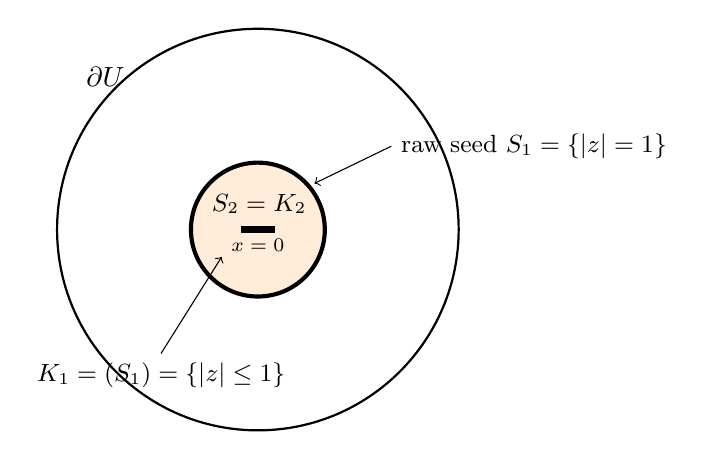
\begin{tikzpicture}[scale=0.85]
% localization boundary
\draw[thick] (0,0) circle (3);
\node at (135:3.22) {$\partial U$};
% filled hull K_1, shaded
\fill[orange!15] (0,0) circle (1);
% raw seed S_1
\draw[line width=1.5pt] (0,0) circle (1);
\draw[<-,shorten <=1.5pt] (40:1.03) -- (32:2.35)
  node[right,align=left] {\small raw seed $S_1=\{|z|=1\}$};
% shaded-hull annotation
\draw[<-,shorten <=1.5pt] (215:0.62) -- (232:2.35)
  node[below,align=left] {\small $K_1=\Fill(S_1)=\{|z|\le1\}$};
% raw seed S_2 inside the hull
\draw[line width=2.6pt] (-0.25,0) -- (0.25,0);
\node[above] at (0.02,0.09) {\small $S_2=K_2$};
% witness point
\fill (0,0) circle (1.3pt);
\node[below,inner sep=2pt] at (0,-0.05) {\scriptsize $x=0$};
\end{tikzpicture}
\caption{The post-fullification merger of Example~\ref{ex:merger} in the
localization $U=\{|z|<3\}$. The raw seeds --- the circle $S_1$ and the segment
$S_2$ --- are disjoint, so every seed-level disjointness audit passes. But the
completion $K_1=\Fill(S_1)$ is the closed unit disk (shaded), which contains
$S_2=K_2$: the completed packets merge. The witness point $x=0$ carries the record
$(1,2,0,\mathrm{ch}_1(0),\mathrm{ch}_2(0))$ with $\mathrm{ch}_1(0)$ the bounded
complementary chamber $\{|z|<1\}$ of $S_1$ and $\mathrm{ch}_2(0)=\textsf{seed}$. By
monotonicity of $\Fill$ the merger persists under every same-label enlargement of
the seeds; only a different typed assignment removes it.}
\label{fig:merger}
\end{figure}

\subsection{The cellwise certificate}\label{subsec:E-cellwise}

The audit clauses of Theorem~\ref{thm:audit} still require computing each completion
and comparing every pair of completions across the localization. The final result of
this section decomposes even this: it confines each packet to its own closed Jordan
cell, inside which the completion is trapped automatically and the port verification
becomes local to the cell. Disjointness of the completions then follows from
disjointness of the cells, which is checked on $N$ disks rather than on
$\binom N2$ pairs of filled hulls.

\begin{proposition}[Cellwise packet-and-port certificate; manuscript Proposition
10.15]\label{prop:cellwise}
Let $U$ be a Jordan domain and let $D_1,\dots,D_N\Subset U$ be pairwise disjoint
closed Jordan disks. Suppose every packet has a compact connected raw seed
$S_\ell\Subset D_\ell$, the seeds cover the complete frozen inventory, and every
original atom $A_i\subset S_i$ has an unprotected point $x_i\in A_i\setminus P_i$
and a Jordan arc $\gamma_i\colon[0,1]\to D_i$ satisfying
\begin{equation}\label{eq:E-arc-condition}
\gamma_i(0)=x_i,
\qquad
\gamma_i\bigl((0,1)\bigr)\subset D_i\setminus S_i,
\qquad
\gamma_i(1)\in\partial D_i
\end{equation}
(condition~(9.11a) of \cite{MWman}). Then $K_\ell=\Fill(S_\ell)\Subset D_\ell$, the
completed packets are pairwise disjoint, every $x_i\in\Exp(A_i,K_i;P_i)$, and the
packet system has simultaneous ports, one common free component, and a protected
regulated connector.
\end{proposition}

\begin{proof}
\emph{Step 1: the completion is trapped in its cell.}
Fix $\ell$. By the Schoenflies theorem, $S^2\setminus D_\ell$ is an open Jordan disk
containing $\infty$, so its planar part $\C\setminus D_\ell$ --- an open disk with
one point removed --- is connected, and it is unbounded. Since
$S_\ell\Subset D_\ell$ means $S_\ell\subset\Int D_\ell$, the exterior
$\C\setminus D_\ell$ is a connected unbounded subset of $\C\setminus S_\ell$ and
therefore lies in the unbounded component $\Omega_\infty(S_\ell)$. Consequently
every bounded component $B$ of $\C\setminus S_\ell$ is disjoint from
$\C\setminus D_\ell$ --- distinct components of $\C\setminus S_\ell$ are disjoint
--- so $B\subset D_\ell$, and $\Fill(S_\ell)\subset D_\ell$. The containment is
compact: a point $x\in\partial D_\ell$ does not lie in $S_\ell\subset\Int D_\ell$,
and every neighborhood of $x$ meets $\C\setminus D_\ell\subset
\Omega_\infty(S_\ell)$; since the component of $\C\setminus S_\ell$ containing $x$
is open and contains a small ball around $x$, that component meets
$\Omega_\infty(S_\ell)$ and hence equals it, so $x\in\Omega_\infty(S_\ell)$ and
$x\notin\Fill(S_\ell)$. Thus $K_\ell=\Fill(S_\ell)\subset\Int D_\ell$, and being
compact, $K_\ell\Subset D_\ell$. The cells are pairwise disjoint, so the completions
are pairwise disjoint, and $D_\ell\Subset U$ gives $K_\ell\Subset U$.

\emph{Step 2: the arc condition certifies exposure.}
Fix $i$. The point $\gamma_i(1)$ lies on the Jordan curve $\partial D_i$, which
bounds the closed Jordan disk $S^2\setminus\Int D_i$ containing $\infty$ in its
interior. Straightening this disk by the Schoenflies theorem \cite{New51} and taking
the preimage of a radius, we obtain a Jordan arc $\beta$ from $\gamma_i(1)$ to
$\infty$ meeting $D_i$ only at $\gamma_i(1)$. Consider the concatenated set
\[
\Gamma\;:=\;\gamma_i\bigl((0,1]\bigr)\,\cup\,\bigl(\beta\setminus\{\infty\}\bigr),
\]
a connected unbounded subset of $\C$. It is disjoint from $S_i$: the piece
$\gamma_i((0,1))$ lies in $D_i\setminus S_i$ by \eqref{eq:E-arc-condition}; the
point $\gamma_i(1)$ lies on $\partial D_i$, which misses $S_i\subset\Int D_i$; and
$\beta\setminus\{\gamma_i(1),\infty\}$ lies in $\C\setminus D_i\subset
\C\setminus S_i$. A connected unbounded subset of $\C\setminus S_i$ lies in the
unbounded component $\Omega_\infty(S_i)$, so in particular
\[
\gamma_i\bigl((0,1]\bigr)\;\subset\;\Omega_\infty(S_i)
\;=\;\C\setminus\Fill(S_i),
\]
that is, $\gamma_i((0,1])$ misses $K_i$. Since $x_i\in A_i\subset S_i\subset K_i$,
this gives
\[
\gamma_i\cap K_i\;=\;\{x_i\} .
\]
The arc $\gamma_i$ maps into $D_i\subset U$, and $x_i\in A_i\setminus P_i$ by
hypothesis, so $\gamma_i$ is precisely an arc of the form read by
\eqref{eq:E-exposure}: every $x_i\in\Exp(A_i,K_i;P_i)$.

\emph{Step 3: assembly.}
The three audit clauses of Theorem~\ref{thm:audit} now hold: clause~(1), because the
seeds are compact, connected, and cover the complete frozen inventory by hypothesis;
clause~(2), by Step~1; and clause~(3), by Step~2. Lemma~\ref{lem:port-localization}
turns the individual arcs into pairwise disjoint simultaneous port arcs with
positive-parameter parts in the common complement of the completions, and
Theorem~\ref{thm:audit} certifies that the geometric augmented-packet clauses of
Definition~\ref{def:packet} hold for this assignment. Theorem~\ref{thm:common-domain}
then determines one common free component of $\Omfree$ with simultaneous singleton
ports to every original atom and supplies a protected regulated connector.
\end{proof}

This proposition is sufficient only, and we close the section by marking the
boundary of what it proves, in the discipline of Section~\ref{sec:scope}. The
cellwise certificate solves the planar verification problem once the cells
$D_\ell$, the complete seeds $S_\ell$, and the unprotected arcs $\gamma_i$ are
supplied. The actual virtual theorem contemplated by the source manuscript must
still \emph{construct} those cells, complete seeds, and unprotected arcs, and must
transport them through the final Wave horizon; that construction is posed in
\cite{MWman} only as an open problem, it is not addressed by anything in this paper,
and no clause of Theorem~\ref{thm:audit} or Proposition~\ref{prop:cellwise} is
promoted here to a statement about virtual carriers, the Wave horizon, or Mandelbrot
local connectivity.
